%grundlagen.tex

\chapter{Grundlagen}
\label{chapter:gru}

\section{Chromatographie}

Die Chromatographie ist ein Verfahren zur Auftrennung von Stoffgemischen. 
Die Auftrennung erfolgt dabei zwischen zwei sogenannten Phasen, der stationären und der mobilen Phase, welche sich in unterschiedlichen Aggregatzuständen befinden und untereinander nicht mischen. Die Analyte werden bewegen sich dabei durch die chromatographische Apparatur, indem sie von der mobilen Phase mitgenommen werden. Immer wieder geraten sie dabei in Kontakt zur stationären Phase und interagieren mit dieser. Abhängig von den Eigenschaften der verschiedenen Stoffe, werden sie dadurch kürzer oder länger aufgehalten, sodass sich verschiedene Stoffe von einander trennen.

Es existieren viele Varianten der Chromatographie. Eine mögliche Unterscheidung findet durch die dabei verwendeten Aggregatzustände der beiden Phasen statt. Zum einen gibt es die Flüssigchromatographie (LC, engl. Liquid Chromatography),
%\todo{Muss englische Worterklärung kursiv oä?}
bei der die mobile Phase eine Flüssigkeit ist und die stationäre Phase ein Feststoff. 
Bei der Gaschromatographie (GC) ist die mobile Phase ein Gas und es wird zusätzlich nach der stationären Phase unterschieden. Ist diese ein Feststoff, so spricht man von gepackten Säulen. Bei der Kapillartechnik hingegen werden die Trennsäulen innen mit einem Flüssigkeitsfilm als stationäre Phase beschichtet.

% Die Gaschromatographie (GC) ist ein Verfahren, mit dem gasförmig vorliegende Stoffgemische aufgetrennt oder analysiert werden können. 
% Die Auftrennung erfolgt dabei zwischen zwei sogenannten Phasen, der stationären und der mobilen Phase, welche sich in unterschiedlichen Aggregatzuständen befinden und untereinander nicht mischen. 

% Allgeinprinzip: Phasen, Phasenwechsel
% Arten der Chroma -> Interessant GC mit Kapillartechnik
% Detektion / Weiterverarbeitung
% Probleme: Peakshapes (Tailing), Ursache
% Verwandte Arbeiten?
% Wo kommt das mit den Referenzdatensätzen rein?

Beispielsweise kann die GC in einer Multikapillarsäule (MCC, engl. Multi Capillary Colum) stattfinden. Sie besteht aus ca. 1000 bis 2000 einzelnen Kapillaren \citep{obinski1999, Baumbach2009}. Jede davon ist innen mit der stationären Phase beschichtet. Außerdem kommt ein Trägergas, die mobile Phase, zum Einsatz, welches die Analyte durch die Säule transportiert. Dieses kann beispielsweise Stickstoff, Helium \citep{obinski1999} oder Luft sein \citep{Baumbach2009}.

\subsection{Der chromatograpische Prozess}
Die nachfolgende Beschreibung des chromatographischen Prozesses bezieht sich auf die Gaschromatographie in Kapillarsäulen. Die prinzipielle Auftrennung der Stoffe durch häufigen Wechsel zwischen den beiden Phasen, ist aber allen Arten der Chromatographie gemein.
\todo{weitere Quelle zum ausführlichen Nachlesen}
Ausführlich beschrieben wurde der chromatograpische Prozess beispielsweise von \cite {kolb2003}.
Die für diese Arbeit wesentlichen Punkte sind hier kurz zusammengefasst:

Die Substanzen unterscheiden sich vor allem durch ihre Wechselwirkungen mit der stationären Phase. Während dieser Wechselwirkungen haften die Teilchen an der stationären Phase, bewegen sich also nicht fort. Finden verhältnismäßig wenig Wechselwirkungen statt, passieren die Teilchen die Säule schneller, als wenn viele Wechselwirkungen stattfinden. Dies beeinflusst die so genannte Retentionszeit, also die Zeit, die zum Durchlaufen der Säule gebraucht wird.

Dabei existieren verschiedene Arten von Wechselwirkungen zwischen den Analytteilchen und der stationären Phase. Zum Einen die Adsorption, bei der die Teilchen mit der Oberfläche der stationären Phase in Kontakt kommen und sich dort anreichern. Die Adsorption findet dabei auf Grund von physikalischen Kräften wie der Van-Der-Waals-Kräften statt. Dadurch ist die Bindung der Stoffe an die stationäre Phase nicht sehr fest und die Teilchen können sich leicht wieder daraus lösen.

Zum Anderen können sich die Analyte aber auch in der stationären Phase lösen. Gelöste Teilchen trennen sich schwerer als adsorbierte Teilchen von der stationären Phase. Die Stoffe verweilen dadurch durchschnittlich länger in der stationären Phase und ihre Durchschnittsgewschindigkeit sinkt.

Auf die eine oder andere Weise diffundieren die Teilchen nun zwischen den beiden Phasen hin und her, wodurch sich ein Gleichgewicht zwischen den Phasen einstellt. Durch dieses Gleichgewicht wandern die Teilchen eines Stoffes als Pulk durch die Säule, bis sie diese verlassen. Für Teilchen vorne im Pulk besteht nur die Möglichkeit, in Wechselwirkung mit der stationären Phase zu treten, bis sich eine Sättigung einstellt. Später ankommmende Teilchen können nur dann in Wechselwirkung treten, wenn bereits wieder Teilchen mobil geworden sind, wodurch sich das Gleichgewicht aufrecht erhält. 
Je nach Verweildauer der einzelnen Teilchen in der stationären Phase, ergibt sich eine für diesen Stoff charakteristische Durchschnittsgeschwindigkeit.%TODO, die den Zeitpunkt der höchsten Austrittsintensität bestimmt.


\subsection{Detektion}
Nach Durchlaufen der Säule wird detektiert, welche Menge an Substanzen austritt. Dabei wird nicht die Art des Analyts festgestellt, sondern nur die Menge der zum jeweiligen Zeitpunkt austretenden Stoffe. Während sich die meisten Stoffe ausreichend in ihrem Verhalten zur stationären Phase unterscheiden und dadurch aufgetrennt die Säule verlassen, kann es aber durchaus vorkommen, dass sich zwei Stoffe hinreichend ähnlich sind und  zumindest teilweise überlappend austreten.

Zur Detektion existieren mehrere Möglichkeiten. Zum Einen kann ein Detektor wie beispielsweise ein Wärmeleitfähigkeitsdetektor oder Flammenionisationsdetektor ein Chromatogramm aufzeichen. Dabei wird in bestimmten Zeitintervallen die austretende Menge Analyte festgestellt. 
%Beispielhaft ist ein Chromatogramm in Abbildung \ref{chromatogramm} zu sehen. 
In Abbildung \ref{chromatogramm} ist ein Beispiel für ein Chromatogramm zu sehen, welches aus mehreren simulierten Daten und Hintergrundrauschen erstellt wurde.
Typischerweise sind zu Beginn einer Messung die Peaks sehr schmal und werden mit zunehmender Retentionszeit eher breiter.
\todo{neues chroma mit breiter werdenden peaks}
%\todo{Bild Chromatogramm (zb ein verrauschter plot 2-3 stoffe, dabei unterschiedlichen pd)}

\begin{figure}
 \centering
  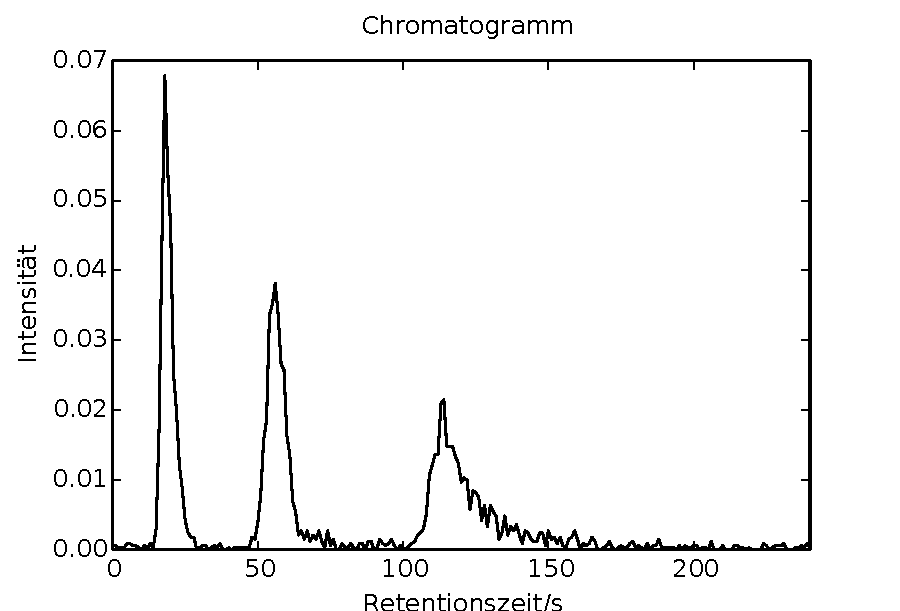
\includegraphics[width = 0.75\textwidth]{bilder/spektrum}\\
  \caption{Beispiel für ein Chromatogramm}
  \label{chromatogramm}
\end{figure}

Alternativ kann die Gaschromatographie auch als Vorverarbeitung für Verfahren wie Massenspektrometrie (MS) oder Ionen-Mobilitäts-Spektrometrie (IMS) dienen. Auch bei diesen Technologien können nicht in jedem Fall alle Stoffe voneinander unterschieden werden. Zum Beispiel existieren Isomere, also Moleküle gleicher Masse aber unterschiedlicher Struktur, die von der MS nicht unterschieden werden können. Durch zuvor statt findende GC jedoch wird nach einer weiteren Stoffeigenschaft unterschieden, sodass diese ähnlichen Stoffe durch die Vortrennung zu verschiedenen Zeitpunkten mit dem zweiten Analyseverfahren beginnen und so doch getrennt im resultierenden Spektrum erscheinen. Wenn eine solche Weiterverarbeitung statt finden soll, werden die aus der MCC austretenden Moleküle direkt ionisiert und in den entsprechenden Geräten weiter analysiert.
Die Kopplung von GC und MS ist beispielsweise von \cite{Hubschmann2009} ausführlich beschrieben worden, näheres zur Kopplung von GC und IMS findet sich zum Beispiel bei \citep{Baumbach2009}. 

%\todo{Wo kann ich sonst Peaks beobachten?}

\subsection{Technische Daten}

Es gibt verschiedene Multikapillarsäulen, die sich in der Anzahl und Größe ihrer Kapillaren, ihrer Länge, ihrer stationären Phase oder der maximalen Temperatur und Druck mit denen sie betrieben werden können, unterscheiden können. Dadurch können sie auch ein unterschiedliches Gasvolumen aufnehmen und trennen und die Durchlaufzeiten für eine Analyse variieren entsprechend. Außerdem können mit ein und derselbsen Säule verschiedene Betriebsmodi verwendet werden, die sich beispielsweise durch verwendetem Druck und damit in der Geschwindigkeit des Trägergases oder der Temperatur unterscheiden. Damit können bei gleichen Analyten sehr unterschiedlich aussehende Chromatogramme erzeugt werden, da die Stoffe auch unterschiedlich auf solche Veränderungen reagieren.

Um eine Einschätzung für eine MCC zu geben, sind hier einige mögliche Daten angegeben. Weitere Spezifikationen finden sich beispielsweise auf der Webseite des Herstellers Multichrom Ltd. \footnote[1]{http://www.mcc-chrom.com/catalogue} \footnote[2]{http://www.mcc-chrom.com/species} 


Eine MCC besteht aus ca. $1000\,$--$\,2000$ Kapillaren mit je $20\,$--$\,80$\,\textmu m Durchmesser. Damit ist sie etwa $2\,$--$\,6$\,mm dick. Die Länge beträgt etwa  $20\,$--$\,40 $\,cm. Die stationäre Phase ist ein Flüssigkeitsfilm, der als ca. $0,1\,$--$\,0,8$\,\textmu m dicke Beschichtung auf die Innenseite der Kapillaren aufgebracht ist. 

Der Querschnitt einer MCC ist in Abbildung \ref{MCC} zu sehen.

\begin{figure}[h]
 \centering
  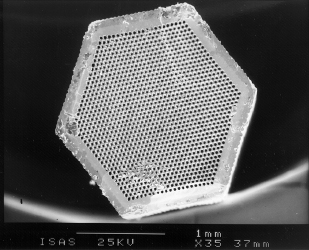
\includegraphics[width = 0.5\textwidth]{bilder/MultiCapillaryColumn}\\
  %\caption[Querschnitt einer MCC]{Querschnitt einer MCC \protect\footnotemark}
  \caption[Querschnitt einer MCC]{Querschnitt einer MCC, Quelle: http://yas.yanaco.co.jp/products/import-gc-ims.html}
  \label{MCC}
\end{figure}
%\footnotetext{http://yas.yanaco.co.jp/products/import-gc-ims.html}

\section{Peakcharakteristika}
Die im gaschromatographischen Experiment gewonnenen, sowie später auch die simulierten Peaks müssen durch einige Eigenschaften beschrieben werden, um sie vergleichbar zu machen. Dafür seien hier drei solcher Eigenschaften beschrieben, die Lage, Breite und Form eines Peaks.

%Um später die simulierten Peaks mit denen aus den Referenzdatensätzen gut vergleichen zu können, sollen nun einige Eigenschaften aufgeführt werden, die einen Peak beschreiben.

\subsection{Lage}
Die offensichtlichste Eigenschaft eines Peaks ist seine Lage, genauer gesagt, die Lage seines Maximums. Je nach verwendeter Technologie unterscheiden sich die Messzeiträume für einen chromatographischen Durchlauf stark voneinander. %\todo{Beispielintervalle}
Allerdings gibt es immer einen minimalen Zeitraum der nach Start der Chromatographie vergangen sein muss, bis ein Peak überhaupt auftreten kann. Dieser hängt von der Geschwindigkeit der mobilen Phase ab, da sich die Analyte nicht schneller als die mobile Phase fortbewegen können und daher mindestens dieselbe Zeit benötigen. Außerdem kann für jede einzelne Messung ein Maximalzeitpunkt gewählt werden, nach dem das Experiment beendet wird.
Für die Gaschromatographie in Multikapillarsäulen liegen die Retentionszeiten typischerweise bei wenigen Sekunden bis Minuten.
%\todo{Ende der Simulation hier festlegen?}


\subsection{Breite}
Peaks können unterschiedlich breit sein. Dabei ist zu beobachten, dass schnelle Teilchen Peaks zu frühen Zeitpunkten erzeugen, die eine relativ geringe Varianz aufweisen, hingegen spätere Peaks tendenziell breiter werden.
% 10% der peakhöhe: kolb, s33. allerdings als tailingfaktor, entspricht eher der schiefemessung
Da jedoch ein Peak mit größerer Intensität, also möglicherweise größerer Stoffmenge, automatisch auch einen höheren und damit breiteren Peak erzeugt, kann die Halbwertsbreite als Maß für die Peakbreite herangezogen werden. Die Halbwertsbreite wird auf halber Maximalhöhe des Peaks gemessen. Im Fall von auftretendem Tailing ist dieser Wert jedoch wahrscheinlich nicht mehr aussagekräftig. Außerdem ist die Halbwertsbreite kein robustes Maß für die Breite, sodass statt dessen der Interquartilsabstand (IQR, engl. interquartile range) als Maß für die Breite verwendet werden kann. Auch dieses Maß ist unabhängig von der Stoffmenge, die den Peak verursacht hat. 
\todo{Quantil, $Q_p$, Quartil definieren}

Der IQR ist entspricht der Differenz zwischen den Quartilen $Q_{25}$ und $Q_{75}$:
\begin{equation}
IQR = Q_{75} -Q_{25}
\end{equation}

 

 % \todo{Zitat IQR, diesen erkären, warum dieses Mass}
\subsection{Form}
Als dritte Eigenschaft können sich Peaks in ihrer Form unterscheiden. Im theoretischen Idealfall haben sie die Form einer Gaußkurve. %\todo{Quelle}
Abweichend davon treten in echten Messungen häufig asymmetrische Peaks auf, die dann ein Tailing aufweisen, diese Eigenschaft wird auch Rechtsschiefe genannt. Dabei steigt die Kurve zunächst stark an, sinkt jedoch nach Erreichen des Maximalwerts deutlich langsamer ab, es entsteht ein Schwanz (engl. Tail).
Ursachen für solche schiefen Peaks gibt es viele \citep{kolb2003, Moretti2004, Giddings1963}. Einige Beispiele für Ursachen sind zusätzliche Adsorptionseffekte, die beim Altern einer Säule auftreten, technische Ursachen wie kleinste Hohlräume zwischen der Säule und dem Gaseinlass bzw. -austritt, sowie einige Stoffe, die generell zu Tailing neigen. %\todo{Zitat, dass einige Stoffe gererell tailen}. 

Als Maß für die Schiefe bietet sich der Quantilskoeffizient \citep{johnson1994} an.
Dieser berechnet sich, aus den Quantilen einer Verteilung und ist definiert als: 
\begin{equation}
\frac{Q_{\alpha} + Q_{1-\alpha} -2\cdot Q_{50} }{ Q_{1-\alpha} - Q_{\alpha}}
\end{equation}

Für $\alpha = 25$ spricht man auch vom Quartilskoeffizienten nach Yule-Bowley und dieser soll später als Maß für die Schiefe der Peaks verwendet werden.


\section{Probabilistische Arithmetische Automaten}
Um die Multikapillarsäule zu simulieren, werden verschiedene Vorgehensweisen angewendet. Am naheliegendsten erscheint es, den chromatographischen Prozess für eine gewisse Anzahl an Teilchen zu simulieren und dabei für jedes einzelne dieser Teilchen mindestens seinen Ort und seinen Zustand festzuhalten. Diese zufallsbasierte Methode hat jedoch den Nachteil, dass verschiedene Durchläufe zu leicht unterschiedlichen Ergebnissen führen können, insbesondere, wenn zu wenige Teilchen simuliert wurden.
Außerdem sind sehr viele teilchen nötig, um glatte Peaks zu bekommen.

Eine andere Möglichkeit besteht darin, die Teilchen als Wahrscheinlichkeitsmasse zu modellieren und für jeden Ort und Zustand festzuhalten, welcher Teil der gesamten Wahrscheinlichkeitsmasse sich dort befindet.
Eine Möglichkeit die Analyte als eine solche Wahrscheinlichkeitsmasse zu betrachten und dadurch eine exakte Verteilung der Teilchen auf Orte und Zustände zu erhalten, bieten Probabilistische Arithmetische Automaten (PAA).
Ein PAA nach \cite{MHKR} ist ein Modell, mit dem eine Folge zufälliger Operationen beschrieben werden kann. 
Für PAA existieren Algorithmen, welche eine gemeinsame Verteilung von Zuständen und Werten oder auch die Verteilung der Wartezeit für einen Wert berechnen. Wie in Kapitel \ref{chapter:mod} beschrieben wird, können die Modelle zur Simulation einer Multikapillarsäule auch als PAA formuliert werden. 
In dieser Formulierung entspricht der Wert auf den gewartet wird, der Länge der Säule und die Zeit, die zum Durchlaufen einer Säule gebraucht wird, ist die Wartezeit für diesen Wert. %Deshalb kann ein PAA nützlich sein, um neben der eigentlichen Simulation auch noch eine erwartete Verteilung der Ankunftszeiten der Teilchen zu berechnen. 

Zunächst sei hier eine Definition für den PAA gegeben, anschließend wird der Algorithmus zur Berechnung der Wartezeit beschrieben.
%In diesem Fall ist die Länge der Säule der Wert, auf den gewartet wird und man ist interessiert in der Verteilung der Anzahl der Zeitschritte, die benötigt werden, um die Länge zu erreichen. 
%TODO: Wo soll das rein? Sinnvoll, wenn das zu Beginn erklärt
% Was tut ein PAA

%\subsection{Definition eines PAA}
% Formale Definition

\begin{definition}[PAA]
 Ein Probabilistischer Arithmetischer Automat (PAA) ist ein Tupel
 $ \mathcal{P} = (\mathcal{Q}, q_0, T, \mathcal{V}, v_0, \mathcal{E}, (e_q)_{q\in\mathcal{Q}}, (\theta_q)_{q\in\mathcal{Q}})$, dabei ist:
 \begin{itemize}
  \item $\mathcal{Q}$ eine endliche Menge von Zuständen
  \item $q_0 \in \mathcal{Q}$ der Startzustand
  \item $T: \mathcal{Q} \times \mathcal{Q} \rightarrow [0,1]$ eine Übergangsfunktion mit $\sum_{q' \in \mathcal{Q}} T(q, q') = 1 $ das heißt $(T(q,q'))_{q,q' \in \mathcal{Q}}$ ist eine stochastische Matrix
  \item $\mathcal{E}$ eine endliche Menge von Emissionen
  \item $e_q: \mathcal{E} \rightarrow [0,1]$ eine Wahrscheinlichkeitsverteilung der Emissionen für jeden Zustand
  \item $\mathcal{V}$ eine Menge von Werten
  \item $v_0$ der Startwert
  \item $\theta_q: \mathcal{V} \times \mathcal{E} \rightarrow \mathcal{V}$ eine Operation für jeden Zustand
 \end{itemize}
\end{definition}
Dabei entspricht $ \mathcal{P} = (\mathcal{Q}, q_0, T)$ einer Markovkette und $ \mathcal{P} = (\mathcal{Q}, q_0, T, \mathcal{E}, (e_q)_{q\in\mathcal{Q}})$ einem Hidden Markov Model. %\todo{Muss ich dann Markov erklären?}
Zusätzlich gibt es für jeden Zustand eine Operation $\theta$, wie beispielsweise Addition oder Subtraktion. Mit Hilfe dieser Operation berechnet sich in jedem Schritt $t$ der neue Wert $v_t$ aus dem Wert des vorherigen Schrittes $v_{t-1}$ und der Emission des aktuellen Zustandes.

Ein PAA ist zu jedem Zeitpunkt mit einer bestimmten Wahrscheinlichkeit in jedem Zustand und kann dabei mit einer bestimmten Wahrscheinlichkeit jeden Wert annehmen. Es existiert also zu jedem Zeitpunkt eine Zustands-Werte-Verteilung. Ausgehend von einer gegebenen Startverteilung, bei dem sich die gesamte Wahrscheinlichkeitsmasse in Zustand $q_0$ befindet und den Wert $v_0$ hat, wird diese Verteilung schrittweise aktualisiert. Dabei findet jeder Übergang gemäß der Wahrscheinlichkeit aus $T$ statt. %Wenn sich der Automat mit der Wahrscheinlichkeit $p$ in Zustand $q$ befindet, 

% 
% wahrscheinlichkeit für neuen Zustand $q'$ ausgehend von allen Zuständen $q$
% 
% $ P(q_n'\mid q_{n-1} ) = (T_{q, q'} \cdot  P(q_{n-1}))$
% 
% $ P(q_n' ) = \sum_q (T_{q, q'} \cdot  P(q_{n-1})$
% Gebe eher p(Q) an

\subsection{Algorithmus zur Berechnung der Wartezeit}

Neben der eben vorgestellten schrittweisen Berechnung der Zustand-Werte Verteilung kann es von Interesse sein, die Verteilung der Wartezeit auf einen bestimmten Wert $v^*$ zu kennen. Für die Teilchen in der MCC entspricht dieser Zielwert der Länge der Säule und man ist interessiert in der Verteilung der Anzahl der Schritte die zum Durchlaufen dieser Strecke benötigt werden. 

Da es sein kann, dass in einigen Abfolgen von Zuständen, der Wert $v^*$ erst sehr spät oder gar nicht erreicht werden kann, wird eine maximale Wartezeit $t_{max}$ gesetzt. Zwar können dann Wartezeiten für $v^*$ größer als $t_{max}$ auftreten, deren genaue Verteilung unbekannt ist, Gesamtwahrscheinlichkeit dieser Zeitpunkte kann jedoch berechnet werden.
% TODO Wohin damit? Es kann sein, dass Wartezeiten für $v^*$ größer als $t_{max}$ auftreten. Dann ist die Verteilung der Wahrscheinlichkeiten für diese Zeitpunkte zwar unbekannt, aber die Gesamtwahrscheinlichkeit für solche Wartezeiten kann berechnet werden.% (teilchen bleiben ewig stecken) aber uns interessiert nur bis zeitpunkt y. (y=240s). Dann kennt man die verteilung darüber hinaus nicht, aber die gesamtwkeit dafür schon.

Außerdem können innerhalb eines Prozesses mehrere Zeitpunkte existieren, an denen der Wert $v^*$ angenommen werden kann, gesucht ist der kleineste dieser Zeitpunkte. %(bspw, wenn Teilchen grad stecken geblieben ist, rein theoretisch) 
Daher kann die Wartezeit auch als Zufallsvariable aufgefasst werden, die definiert als: $W_{v^*} = \min\{t \in \mathbb{N}\mid v_t = v^*\}$.
%Warte auf Wert $v^*$: 
%Gesucht ist der minimale Zeitpunkt $t$, an dem $v_t$ den Wert $v^*$ angenommen hat. 
%Die Wartezeit ist eine Zufallsvariable, definiert als: $W_{v^*} = \min\{t \in \mathbb{N}\mid v_t = v^*\}$

Wie oben beschrieben, existiert die Möglichkeit, die Zustands-Werte Verteilung schrittweise für alle Zeitpunkte bis zu einem gewünschten Maximalzeitpunkt $t_{max}$ zu berechnen.
Gesucht ist nun die Verteilung über die Zeitpunkte $t < t_{max}$ für einen Zielwert $v^*$. $P(v_{t} = v^*)$ ist die Wahrscheinlichkeit für jeden solchen Zeitpunkt $t$, $v^*$  zu erreichen. Dies entspricht der Summe über alle Zuständen, die zu Zeitpunkt $t$ den Wert $v^*$ erreichen können. Also ist $P(v_t = v^*)  = \sum_{q \in \mathcal{Q}} P(q_{t} = q, v_{t} = v^*)$


Zur Berechnung der Verteilung der Wartezeit auf $v^*$ wird ein modifizierter PAA konstruiert. Hierbei werden zwei neue Zustände eingeführt, $\bullet$ und $\circ$, sodass der neue PAA die Zustände $\mathcal{V}' = \mathcal{V} \cup \{\bullet, \circ\}$ hat. Außerdem werden die Operationen angepasst auf

$ \theta'_q(v,e)=
\begin{cases}
\theta_q(v,e), 	& \text{wenn } v \notin \{\bullet, \circ\} \text{ und } \theta_q(v,e) \neq v^* ,\\
\bullet,	& \text{wenn } v \notin \{\bullet, \circ\} \text{ und } \theta_q(v,e) = v^* ,  \\
\circ, 		& \text{wenn } v \in \{\bullet, \circ\}
\end{cases}$.

Der Wert $\bullet$ wird also genau dann erreicht, wenn im aktuellen Berechnungsschritt die ursprüngliche Operation den Zielwert $v^*$ erreicht. Also gilt für alle Zeiten $t < t_{max}$: $P(W_{v^*} = t) = P(v'_t = \bullet)$.

Die Verteilung für $P(v'_{t} = \bullet)$ kann wie oben angegeben schrittweise für alle Zeitpunkte $t$ ausgehend von der Startverteilung bis zu $t_{max}$ berechnet werden. Dadurch, dass im jeweils nächsten Berechnungsschritt der PAA in Zustand $\circ$ gelangt, wird jeweils nur das erste Erreichen von $v^*$ berücksichtigt.

Durch Berechnung der Wahrsscheinlichkeiten $P(v'_{t} = \bullet)$ für alle $t < t_{max}$ erhält man die Verteilung der Wartezeiten auf $v^*$.

%Offensichtlich entspricht die Wartezeit auf den Wert $v^*$ der Wahrscheinlichkeit von Wert $\bullet$
%Es kann also für alle Zeitpunkte $t$ die Wahrscheinlichkeit für den neuen Wert $\bullet$ berechnet werden.
%TODO